\documentclass[a4paper,10pt,onecolumn]{article}
\usepackage{amsmath}
\usepackage{framed}
\usepackage{graphicx}

\setlength\parindent{0pt} % Remove automatical indent for new paragraph

\begin{document}

\title{Practical Programming Exam - Exercise 20 and question 11.3}
\author{Jonas Hjorth Knudsen\\ 201406333}
\date{\today}

\maketitle



\section{Question 3 from lecture 11}

\textit{Suppose you run the command \emph{make main} and it fails with diagnostics}

\begin{framed}
cc \hspace{1cm} main.c \hspace{1cm} -o main\\
main.c:1:19: fatal error: gsl\_sf.h: No such file or directory\\
compilation terminated.
\end{framed}

\textit{Explain the error and how to correct it.}\\

The error occur because the header in main.c is wrong. The headerfile is \#include\textless gsl\_sf.h\textgreater
 when it should be \#include\textless gsl/gsl\_sf.h\textgreater.
The reason for haveing gsl/... is because the gsl library files are installed in their own directory called gsl.



\section{Exercise 20}






\section{Exercise 32}

\begin{figure}
	\centering
	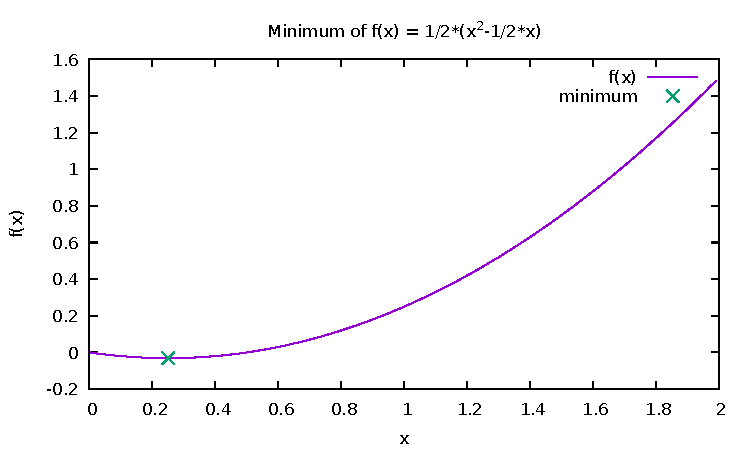
\includegraphics{plotMin.pdf}
	\caption{Minimum of the function $f(x) = \frac{1}{2} (x^2-\frac{1}{2}x)$}
	\label{fig:min}
\end{figure}


\end{document}
